\documentclass{scrartcl}
\usepackage[latin1]{inputenc}
\usepackage{tikz}
\usepackage{pgf-umlcd}
\usepackage{amssymb}
%\setkomafont{disposition}{\normalfont\bfseries}




\begin{document}

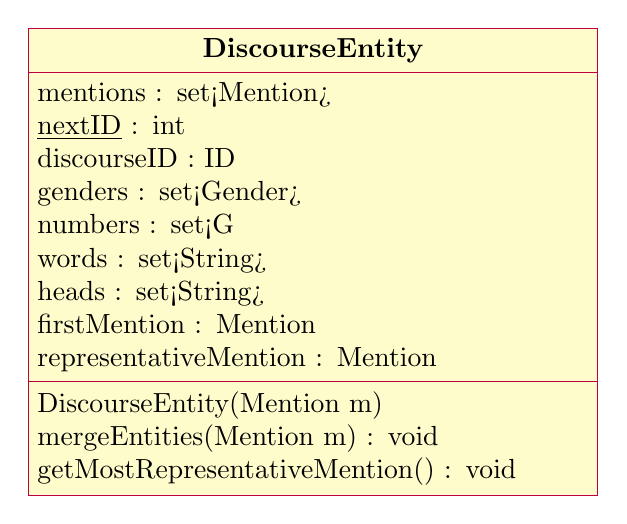
\begin{tikzpicture}
  \begin{class}[text width=7cm ]{DiscourseEntity}{0,0}
  	\attribute{mentions : set<Mention>}
  	\attribute{\underline{nextID} : int}
  	\attribute{discourseID : ID}
    \attribute{genders : set<Gender>}
    \attribute{numbers : set<G}
	\attribute{words : set<String>}
	\attribute{heads : set<String>}
	\attribute{firstMention : Mention}
	\attribute{representativeMention : Mention}
    \operation{DiscourseEntity(Mention m)}
    
    \operation{mergeEntities(Mention m) : void}
    \operation{getMostRepresentativeMention() : void}
  \end{class}
\end{tikzpicture}
\bigskip


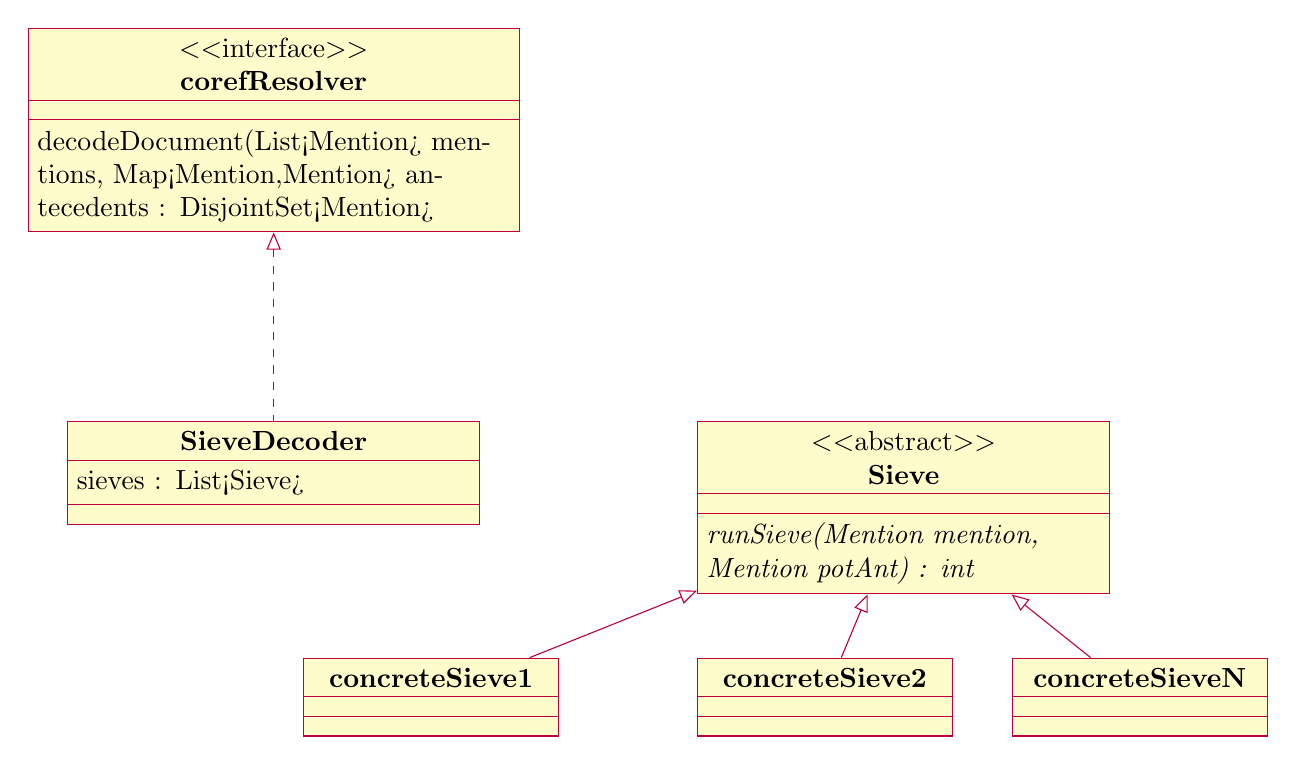
\begin{tikzpicture}
  \begin{interface}[text width=6cm]{corefResolver}{0,0}  	
    \operation{decodeDocument(List<Mention> mentions, Map<Mention,Mention> antecedents : DisjointSet<Mention>}
  \end{interface}
  
  \begin{class}{SieveDecoder}{0,-5}    
    \implement{corefResolver}
    \attribute{sieves : List<Sieve>}
  \end{class}
  
  \begin{abstractclass}{Sieve}{8,-5}
    \operation[0]{runSieve(Mention mention, Mention potAnt) : int}
  \end{abstractclass}
  
  \begin{class}[text width=3cm]{concreteSieve1}{2,-8}
    \inherit{Sieve}
  \end{class}
  
  \begin{class}[text width=3cm]{concreteSieve2}{7,-8}
    \inherit{Sieve}
  \end{class}
  
  \begin{class}[text width=3cm]{concreteSieveN}{11,-8}
    \inherit{Sieve}
  \end{class}
  
\end{tikzpicture}




\end{document}






